\bookchapter{}{The map of the application}{Where, in the simulator, to find everything the lessons refer to: the screen, the keys, the levels, the controllers, every parameter group and the source of each lesson.}
\label{app:map}
% An unlabelled chapter: its figures and tables are numbered 1, 2, … (restored at the end).
\renewcommand{\thefigure}{\arabic{figure}}\renewcommand{\thetable}{\arabic{table}}

% In this appendix a source path may break after any slash: the tables are full of them.
\ExplSyntaxOn
\tl_new:N \l__anem_map_tl
\cs_new_protected:Npn \__anem_map_href:nn #1#2 { \href{\repo#1}{\texttt{\color{deepblue}#2}} }
\cs_generate_variant:Nn \__anem_map_href:nn { nV }
\NewDocumentCommand{\mapsrc}{m}{
  \tl_set:Nn \l__anem_map_tl {#1}
  \tl_replace_all:Nnn \l__anem_map_tl {/} {/\penalty0\relax}
  \__anem_map_href:nV {#1} \l__anem_map_tl
}
\NewDocumentCommand{\tsrc}{m}{
  \tl_set:Nn \l__anem_map_tl {#1}
  \tl_replace_all:Nnn \l__anem_map_tl {/} {/\penalty0\relax}
  \__anem_map_href:nV {src/#1} \l__anem_map_tl
}
\ExplSyntaxOff
% In the tables an on-screen label keeps the size of the table.
\newcommand{\uitab}[1]{\leavevmode{\sffamily\color{ink}#1}}
\let\anemsrcsaved\src
\let\src\mapsrc


\lead{The lessons say \enquote{open the group \ui{Altitude PID}} or \enquote{set the inner stage} and trust the reader to find it. This appendix is the map that makes that possible. Everything in it is read off the code of the simulator as it is; where a name differs between the screen and the source, both are given.}

\begin{inapp}[Starting the simulator]
\texttt{make dev} in the repository serves the app at \texttt{http://localhost:5173}. A lesson is loaded from the lesson panel with \ui{Start}: the parameters return to their defaults, the lesson's changes are applied on top, the run starts from the ground and the charts switch to the lesson's loop.
\end{inapp}

\noindent The book writes the four kinds of thing in the app in four ways. \ui{Group\then Field} is what you see on the screen: a group of the parameter panel, a menu, a button, followed through its menus by \then. \param{control.alt.kp} is the same parameter as the code knows it: its path in the parameter object of \src{src/sim/params.ts}, as listed in \src{src/engine/schema.ts}. That path is also what the share link carries. \key{R} is a key. \src{src/control/pid.ts} is a file of the repository, linked to it in the PDF; in the tables of this appendix the leading \texttt{src/} is left out.

\section*{The screen}

\begin{figure}[tbp]
  \begin{fullwidth}
    \begin{tikzpicture}[mk/.style={circle, fill=accent, draw=white, line width=0.6pt, text=white,
        inner sep=0pt, minimum size=4.2mm, font=\sffamily\bfseries\scriptsize}]
      \node[anchor=south west, inner sep=0pt] (img) {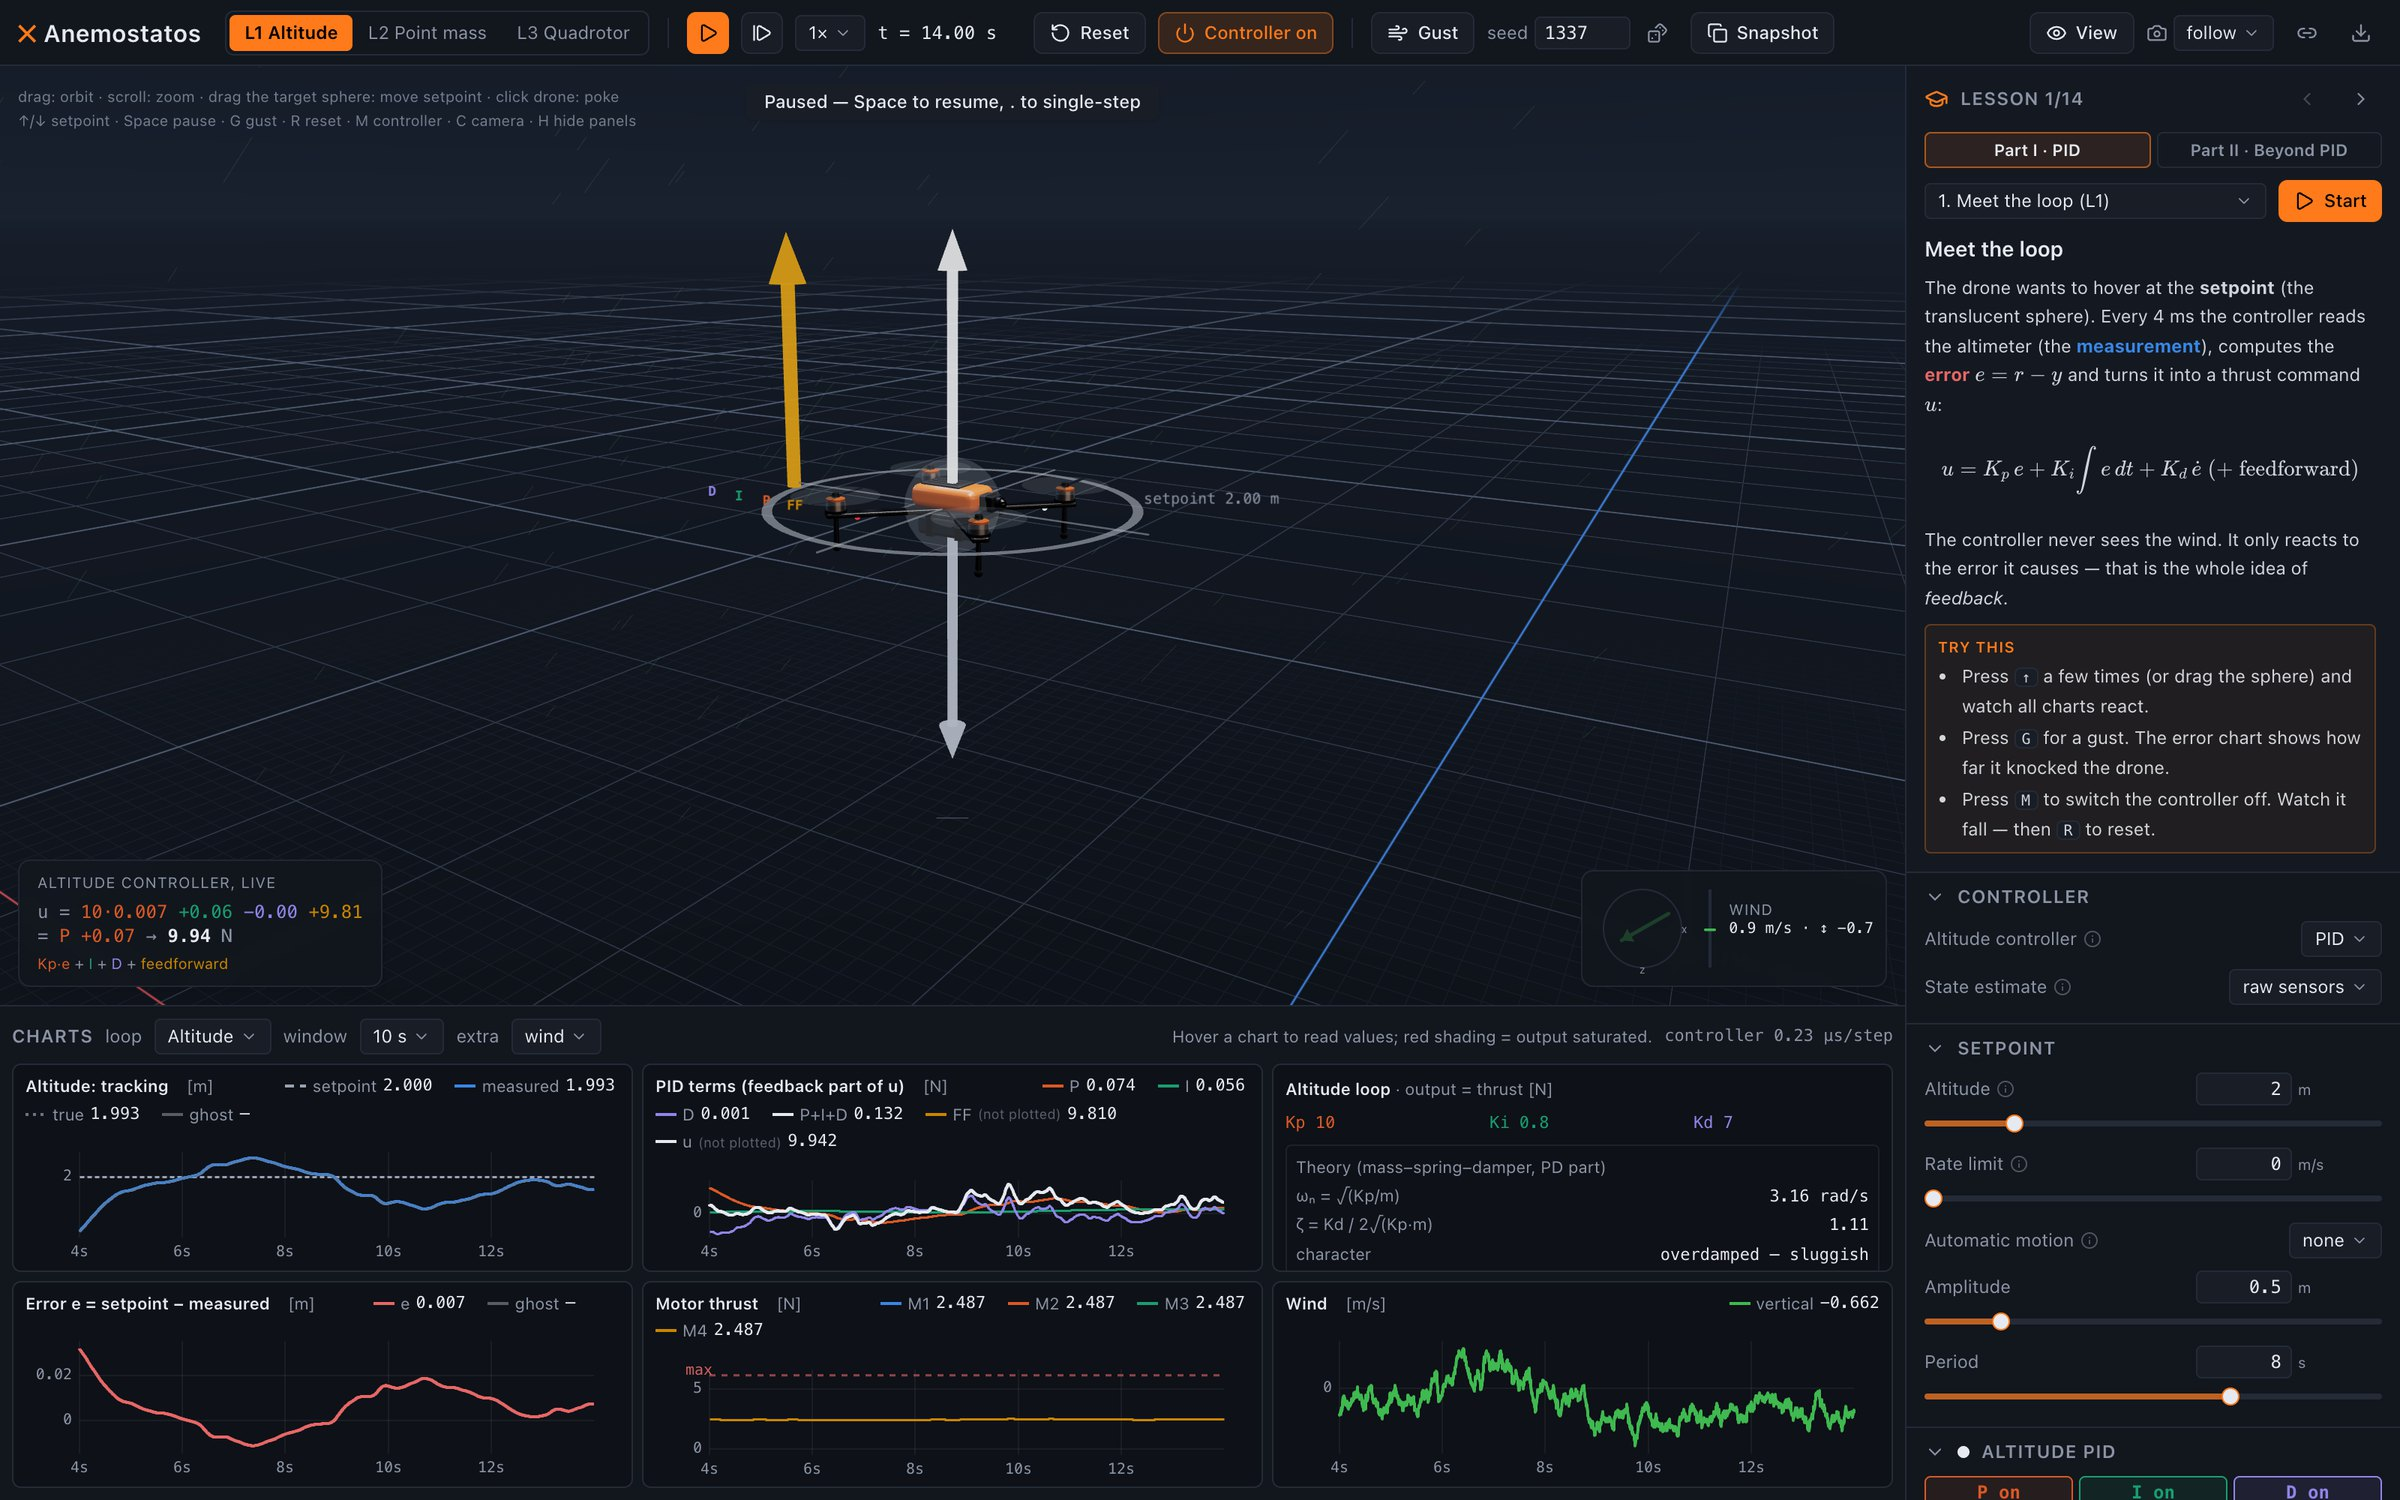
\includegraphics[width=\linewidth]{screens/meet}};
      \begin{scope}[x={(img.south east)}, y={(img.north west)}]
        \node[mk] at (0.183,0.940) {1};
        \node[mk] at (0.300,0.940) {2};
        \node[mk] at (0.584,0.940) {3};
        \node[mk] at (0.735,0.940) {4};
        \node[mk] at (0.900,0.945) {5};
        \node[mk] at (0.285,0.910) {6};
        \node[mk] at (0.493,0.890) {7};
        \node[mk] at (0.545,0.700) {8};
        \node[mk] at (0.168,0.392) {9};
        \node[mk] at (0.648,0.392) {10};
        \node[mk] at (0.806,0.934) {11};
        \node[mk] at (0.784,0.402) {12};
        \node[mk] at (0.256,0.312) {13};
        \node[mk] at (0.030,0.270) {a};
        \node[mk] at (0.292,0.270) {b};
        \node[mk] at (0.554,0.270) {c};
        \node[mk] at (0.030,0.125) {d};
        \node[mk] at (0.292,0.125) {e};
        \node[mk] at (0.554,0.125) {f};
      \end{scope}
    \end{tikzpicture}
    \caption{The screen of Anemostatos, its parts numbered as in \cref{tab:map-screen}. The screen is a grid: the toolbar across the top, the 3D view, the side panel on the right (lessons above, parameters below) and the six charts underneath. \key{H} hides the side panel and the charts and leaves the 3D view alone.}
    \label{fig:map-screen}
  \end{fullwidth}
\end{figure}

\Cref{fig:map-screen} is the screen during Lesson~I.1, and \cref{tab:map-screen} names its parts. The layout itself is in \src{src/App.tsx}: a toolbar \SI{44}{px} high, a side panel \SI{330}{px} wide and a chart area \SI{330}{px} high around the 3D view.

\begin{table}[tbp]
\begin{fullwidth}\footnotesize\let\ui\uitab
\renewcommand{\arraystretch}{1.22}
\begin{tabularx}{\linewidth}{@{}>{\sffamily\bfseries\color{accent}}l>{\raggedright}p{36mm}>{\raggedright\arraybackslash}X>{\raggedright\arraybackslash}p{37mm}@{}}
\toprule
 & \normalfont\sffamily part & \sffamily what it does & \sffamily source\\
\midrule
1 & \ui{L1 Altitude · L2 Point mass · L3 Quadrotor} & The level (\cref{tab:map-levels}). Changing it restarts the run. Keys \key{1} \key{2} \key{3}. & \tsrc{ui/Toolbar.tsx}\\
2 & pause, single step, speed, clock & Pause or resume (\key{Space}); one controller period forward while paused (\key{.}); simulation speed $0.1\times$ to $4\times$; the simulated time $t$. & \tsrc{ui/Toolbar.tsx}\\
 & \ui{Reset}, \ui{Controller on} & Restart from the ground with the current parameters (\key{R}); switch the controller off, motors idle, and on again (\key{M}). & \tsrc{engine/simulation.ts}\\
3 & \ui{Gust}, \ui{seed} & A strong gust now (\key{G}). The seed of the wind: same seed and same parameters, the same wind to the millisecond; the dice draw a new one. & \tsrc{ui/actions.ts}, \tsrc{sim/wind.ts}\\
4 & \ui{Snapshot} & Freeze the run as a grey \emph{ghost} trace in the charts (\key{S}); change something, press \key{R}, compare on the same wind. A chip \ui{ghost: …} beside it removes the ghost. & \tsrc{ui/actions.ts}\\
5 & \ui{View}, camera & \ui{View}: the 3D overlays \ui{Forces}, \ui{P / I / D arrows}, \ui{Setpoint marker}, \ui{Height ruler}, \ui{Trail}, \ui{Wind tracers}. The camera: \ui{orbit}, \ui{follow} (the default), \ui{side}, \ui{top}; \key{C} cycles. Then: copy a link with every parameter; download the last \SI{60}{s} of telemetry as CSV. & \tsrc{ui/Toolbar.tsx}, \tsrc{scene/CameraRig.tsx}\\
6 & hint line & The mouse and the keys, in one line. & \tsrc{App.tsx}\\
7 & status badges & \ui{Crashed!}, \ui{Controller off}, \ui{Taking off…} (integrators held until airborne), \ui{Paused}, \ui{Simulation slowed down}. & \tsrc{ui/hud/StatusBadges.tsx}\\
8 & 3D view & The drone, the translucent setpoint sphere (drag it), the force arrows in the colours of the terms, the wind tracers. & \tsrc{scene/Scene.tsx}\\
9 & live formula & The controller's output as the sum of its terms, with this instant's numbers; for a controller other than PID, the sum of its named contributions. & \tsrc{ui/hud/LiveFormula.tsx}\\
10 & wind indicator & Direction and speed of the wind at the drone, and its vertical part. & \tsrc{ui/hud/WindHud.tsx}\\
11 & lesson panel & Parts I–IV, the lesson list with its level, \ui{Start}, the text and its \emph{Try this}, and the \ui{Goal}, which turns green when reached. Arrows step through the lessons. & \tsrc{lessons/LessonPanel.tsx}\\
12 & parameter panel & Every parameter, in collapsible groups (\cref{tab:map-groups}). & \tsrc{ui/params/ParamPanel.tsx}\\
13 & chart header & \ui{loop}, \ui{window} (\SIlist{5;10;30;60}{s}), \ui{extra}, \ui{beside it}, and the time the controller takes per step. & \tsrc{ui/charts/ChartsPanel.tsx}\\
a–f & the six charts & See \cref{tab:map-charts}. & \tsrc{ui/charts/}\\
\bottomrule
\end{tabularx}
\caption{The parts of the screen, as numbered in \cref{fig:map-screen}.}
\label{tab:map-screen}
\end{fullwidth}
\end{table}

\subsection*{The parameter panel}

Each group of the panel (\cref{tab:map-groups}) folds open with a click on its title; \ui{Controller}, \ui{Setpoint}, \ui{Altitude PID}, \ui{LQR}, \ui{ADRC} and \ui{Kalman filter} start open, and so does \ui{Horizontal PID (X, Z)} above Level~1. A group appears only when it applies: the PID groups when a PID flies, \ui{MPC} when MPC is chosen, a field such as \ui{X} only on the levels that have it, and a choice with a single option not at all. Every number has a slider and a box for typing; the small arrow beside the box returns it to its default, and the \textsf{i} beside a label explains the parameter. In a PID group three coloured buttons, \ui{P on · I on · D on}, switch the terms, and the less common settings, \ui{D acts on}, \ui{D filter}, \ui{Anti-windup}, \ui{I limit} and \ui{Kb}, wait under \ui{Practical details (D filter, anti-windup…)}. Clicking the title of a group that belongs to a loop shows that loop in the charts.

\subsection*{The charts}

The chart area is a grid of three columns and two rows (\cref{tab:map-charts}). The \ui{loop} menu chooses which control loop the four left charts and the card show; \cref{tab:map-levels} lists the loops of each level. Hovering a chart reads its values; a red band means the output of the loop was saturated.

\begin{table}[tbp]
\begin{fullwidth}\footnotesize\let\ui\uitab
\renewcommand{\arraystretch}{1.22}
\begin{tabularx}{\linewidth}{@{}>{\sffamily\bfseries\color{accent}}l>{\raggedright}p{40mm}>{\raggedright\arraybackslash}X@{}}
\toprule
 & \normalfont\sffamily chart & \sffamily what it shows\\
\midrule
a & \ui{\emph{loop}: tracking} & The setpoint (dashed), the measurement, the true value when the sensor lies, and the ghost.\\
b & \ui{PID terms (feedback part of u)} & \Pt, \It, \Dt\ and their sum, with the feedforward and the total $u$ in the legend; for any other controller, \ui{Contributions}.\\
c & info card & The gains, and for the force loops of L1 and L2 the theory of the PD part: $\omega_n$, $\zeta$, the character of the response, the predicted steady-state error, $T_i$ and $T_d$. Below, the step metrics of the last setpoint step: rise time 10–90\,\%, overshoot, settling time $\pm 2\,\%$, steady-state error. A controller other than PID lists what it says about itself (gains, poles, estimates); at L3 a planned trajectory shows the speed, acceleration and tilt it needs (\tsrc{ui/charts/InfoCard.tsx}, \tsrc{ui/charts/StepMetrics.tsx}).\\
d & \ui{Error e = setpoint − measured} & The error of the loop, and the ghost's.\\
e & \ui{Motor thrust} & The four motors, with their maximum. The menu \ui{beside it} replaces it with \ui{Bode plot}, \ui{Nyquist plot}, \ui{pole map} or \ui{filter uncertainty}.\\
f & \ui{extra}: \ui{wind} & The default. Part II uses \ui{disturbance} (the force the model does not explain, true and estimated), \ui{phase portrait} and \ui{estimate vs truth}; the later parts add the analysis charts. A tall chart, such as the Bode plot, takes the whole right column in place of c and f.\\
\bottomrule
\end{tabularx}
\caption{The six charts, lettered as in \cref{fig:map-screen}: top row a, b, c; bottom row d, e, f.}
\label{tab:map-charts}
\end{fullwidth}
\end{table}

\section*{Keys and mouse}

The keys are read in \src{src/ui/useKeyboard.ts} and act anywhere except while typing in a box. The mouse acts on the 3D view: the drone in \src{src/scene/DroneRig.tsx}, the setpoint sphere in \src{src/scene/overlays/SetpointGhost.tsx}.

\begin{center}\small
\renewcommand{\arraystretch}{1.25}
\begin{tabularx}{\linewidth}{@{}>{\raggedright}p{27mm}>{\raggedright\arraybackslash}X@{}}
\toprule
\sffamily key & \sffamily action\\
\midrule
\key{Space} & pause and resume\\
\key{.} & one controller period forward, while paused\\
\key{R} & reset: restart from the ground; a lesson's scripted events replay\\
\key{M} & controller on and off\\
\key{G} & a strong gust now\\
\key{↑}\ \key{↓} & altitude setpoint up or down by \SI{0.1}{m}; with \key{Shift}, by \SI{1}{m} (kept within \SIrange{0.2}{10}{m})\\
\key{1}\ \key{2}\ \key{3} & Level~1, 2 or 3\\
\key{C} & next camera: orbit, follow, side, top\\
\key{S} & snapshot: keep this run as the ghost\\
\key{H} & hide or show the side panel and the charts\\
\midrule
\sffamily mouse & \\
\midrule
drag, scroll & orbit the camera, zoom\\
drag the sphere & move the setpoint: vertically at L1; horizontally at L2 and L3, vertically with \key{Shift}\\
click the drone & a shove: downwards at L1, away from the camera at L2 and L3\\
\bottomrule
\end{tabularx}
\end{center}

\section*{The three levels}

The same drone is simulated at three levels of truth (\cref{tab:map-levels}). The physics always runs at \SI{1}{kHz} (\src{src/engine/simulation.ts}); the controller runs at \ui{Controller rate}, \param{control.rateHz}, \SI{250}{Hz} by default. \param{sim.level} holds the level, and a link made with the toolbar keeps it.

\begin{table}[tbp]
\begin{fullwidth}\footnotesize\let\ui\uitab
\renewcommand{\arraystretch}{1.22}
\begin{tabularx}{\linewidth}{@{}>{\sffamily\bfseries\color{accent}}l>{\raggedright}X>{\raggedright}p{43mm}>{\raggedright\arraybackslash}p{46mm}@{}}
\toprule
 & \normalfont\sffamily the vehicle & \sffamily loops in the charts & \sffamily controllers\\
\midrule
L1 & \textbf{Altitude.} The drone moves only up and down; the four motors push together, the controller chooses the total thrust. & \ui{Altitude} (\texttt{alt}) & \tsrc{control/registry.ts}: one of eleven altitude controllers (\cref{tab:map-controllers}), with or without a Kalman filter\\
L2 & \textbf{Point mass.} Three independent forces push a point in 3D. A cheat: a real drone must tilt. & \ui{Position X, Y, Z} (\texttt{pos.x}, \texttt{pos.y}, \texttt{pos.z}); default \texttt{pos.y} & \tsrc{control/pointmass.ts}: \ui{Altitude PID} on Y, \ui{Horizontal PID (X, Z)} on X and Z\\
L3 & \textbf{Quadrotor.} Six degrees of freedom: four motors with lag, attitude as a quaternion, the cascade position → velocity → attitude → rate → motors. & \ui{Position}, \ui{Velocity}, \ui{Attitude} and \ui{Rate} on each axis (\texttt{pos.x} … \texttt{rate.yaw}), \ui{Accel} with acceleration INDI; default \texttt{pos.y} & \tsrc{control/cascade.ts}, built from the five choices of \cref{tab:map-controllers3}\\
\bottomrule
\end{tabularx}
\caption{The levels. The physics of all three is in \tsrc{sim/dynamics.ts}, the wind in \tsrc{sim/wind.ts} and the sensors in \tsrc{sim/sensors.ts}; the loops are listed in \tsrc{ui/charts/loops.ts}.}
\label{tab:map-levels}
\end{fullwidth}
\end{table}

\section*{The controllers}

What flies is chosen in the group \ui{Controller}, and \src{src/control/registry.ts} builds it; any change of choice restarts the run. \Cref{tab:map-controllers,tab:map-controllers3} list every option by its label on the screen, its value in the parameters and the file that implements it. At L2 there is nothing to choose, and the group is hidden.

\begin{table}[tbp]
\begin{fullwidth}\footnotesize\let\ui\uitab
\renewcommand{\arraystretch}{1.13}
\begin{tabularx}{\linewidth}{@{}>{\raggedright}p{43mm}>{\raggedright}p{27mm}>{\raggedright}X>{\raggedright\arraybackslash}p{25mm}@{}}
\toprule
\sffamily option on the screen & \sffamily value & \sffamily source & \sffamily lessons\\
\midrule
\multicolumn{4}{@{}l}{\sanscaps\scriptsize\color{accent}L1 · ALTITUDE CONTROLLER\quad\normalfont\param{control.l1.kind}}\\
\ui{PID} (default) & \texttt{pid} & \tsrc{control/altitude.ts}, \tsrc{control/pid.ts} & Part I, II.1\\
\ui{LQR / LQI} & \texttt{lqr} & \tsrc{control/lqr.ts} & II.2, II.3\\
\ui{ADRC} & \texttt{adrc} & \tsrc{control/adrc.ts}, \tsrc{estimation/eso.ts} & II.5, II.6\\
\ui{MPC} & \texttt{mpc} & \tsrc{control/mpc.ts}, \tsrc{math/qp.ts} & II.13, II.14\\
\ui{L1 adaptive} & \texttt{l1ac} & \tsrc{control/l1ac.ts} & II.18\\
\ui{H∞ loop shaping}, \ui{sliding mode}, \ui{MRAC (adaptive)}, \ui{backstepping} & \texttt{hinf}, \texttt{smc}, \texttt{mrac}, \texttt{backstepping} & \tsrc{control/hinf.ts}, \tsrc{control/smc.ts}, \tsrc{control/mrac.ts}, \tsrc{control/backstepping.ts} & Part III\\
\ui{bang-bang (time-optimal)}, \ui{dynamic programming} & \texttt{bangbang}, \texttt{dp} & \tsrc{control/bangbang.ts}, \tsrc{control/dp.ts} & Part IV\\
\multicolumn{4}{@{}l}{\sanscaps\scriptsize\color{accent}L1 · STATE ESTIMATE\quad\normalfont\param{control.l1.estimator}}\\
\ui{raw sensors} (default), \ui{Kalman filter} & \texttt{none}, \texttt{kalman} & \tsrc{control/estimated.ts}, \tsrc{estimation/kalman.ts} & II.4\\
\bottomrule
\end{tabularx}
\caption{The controllers of Level~1, chosen in the group \ui{Controller}.}
\label{tab:map-controllers}
\end{fullwidth}
\end{table}

\begin{table}[tbp]
\begin{fullwidth}\footnotesize\let\ui\uitab
\renewcommand{\arraystretch}{1.13}
\begin{tabularx}{\linewidth}{@{}>{\raggedright}p{43mm}>{\raggedright}p{27mm}>{\raggedright}X>{\raggedright\arraybackslash}p{25mm}@{}}
\toprule
\sffamily option on the screen & \sffamily value & \sffamily source & \sffamily lessons\\
\midrule
\multicolumn{4}{@{}l}{\sanscaps\scriptsize\color{accent}L3 · OUTER STAGE\quad\normalfont\param{control.l3.outer}}\\
\ui{PID cascade} (default) & \texttt{pid-cascade} & \tsrc{control/cascade.ts}, \tsrc{control/pid.ts} & I.13, I.14\\
\ui{geometric tracking (Lee)} & \texttt{geometric} & \tsrc{control/geometric.ts} & II.10–II.12\\
\ui{MPC (linear, point mass)} & \texttt{mpc} & \tsrc{control/mpc.ts} & II.15\\
\ui{MPPI (sampling)} & \texttt{mppi} & \tsrc{control/mppi.ts} & II.16\\
\ui{neural network policy} & \texttt{policy} & \tsrc{control/policy.ts}, \tsrc{control/policy-weights.ts} & II.20\\
\multicolumn{4}{@{}l}{\sanscaps\scriptsize\color{accent}L3 · ATTITUDE LAW\quad\normalfont\param{control.l3.attitude}}\\
\ui{quaternion error} (default), \ui{tilt-prioritised}, \ui{Euler angles (naive)} & \texttt{quaternion}, \texttt{tilt}, \texttt{euler} & \tsrc{control/geometric.ts}, \tsrc{math/quat.ts} & II.10\\
\multicolumn{4}{@{}l}{\sanscaps\scriptsize\color{accent}L3 · INNER STAGE\quad\normalfont\param{control.l3.inner}}\\
\ui{attitude P + rate PID} (default) & \texttt{pid} & \tsrc{control/stages.ts} (\texttt{PidRateStage}) & I.13\\
\ui{attitude P + rate INDI} & \texttt{indi} & \tsrc{control/stages.ts} (\texttt{RateIndi}) & II.7, II.9\\
\multicolumn{4}{@{}l}{\sanscaps\scriptsize\color{accent}L3 · DISTURBANCE COMPENSATION\quad\normalfont\param{control.l3.compensation}}\\
\ui{none (m̂·a model)} (default) & \texttt{none} & \tsrc{control/stages.ts} (\texttt{NoCompensation}) & \\
\ui{acceleration INDI} & \texttt{indi} & \tsrc{control/stages.ts} (\texttt{AccelIndi}) & II.8, II.15\\
\ui{L1 adaptive} & \texttt{l1ac} & \tsrc{control/l1ac.ts} (\texttt{L1Compensation}) & II.18\\
\ui{learned residual model} & \texttt{learned} & \tsrc{control/residual.ts} & II.19\\
\multicolumn{4}{@{}l}{\sanscaps\scriptsize\color{accent}L3 · SAFETY FILTER\quad\normalfont\param{control.l3.safety}}\\
\ui{none} (default), \ui{control barrier function} & \texttt{none}, \texttt{cbf} & \tsrc{control/cbf.ts} & II.17\\
\bottomrule
\end{tabularx}
\caption{The controllers of Level~3. The rotor-loss controller of Part III, \tsrc{control/fault.ts}, replaces the PID cascade when \param{control.fault.enabled} is set.}
\label{tab:map-controllers3}
\end{fullwidth}
\end{table}

\section*{The parameter groups}

\Cref{tab:map-groups,tab:map-groups2} list the groups that Parts I and II use, in the order of the panel. A path ending in \texttt{.*} stands for a whole PID: \texttt{kp}, \texttt{ki}, \texttt{kd}, the switches \texttt{pOn}, \texttt{iOn}, \texttt{dOn}, and the practical details \texttt{derivativeOn}, \texttt{dFilterHz}, \texttt{antiWindup}, \texttt{iLimit}, \texttt{kb} (\src{src/control/pid.ts}). The defaults of every parameter are in \texttt{defaultParams} of \src{src/sim/params.ts}.

The groups of the later parts follow in the panel: \ui{Loop shaping}, the groups of the Part~III controllers, \ui{Uncertainty (plant family)}, \ui{Rotor loss}, \ui{Fault monitor}, \ui{Vibration \& IMU}, \ui{Attitude estimate}, \ui{Guidance (chase a target)}, \ui{Inertial navigation \& beacons}, \ui{Navigation}, \ui{Gyro filter}, \ui{Identification (chirp)} and \ui{Probe (frequency response)}, and, when \ui{Physics\then Vehicle} is not the quadrotor, the groups of the rocket, the aircraft and the satellite of Part~IV.

\begin{table}[p]
\begin{fullwidth}\footnotesize\let\ui\uitab
\renewcommand{\arraystretch}{1.12}
\begin{tabularx}{\linewidth}{@{}>{\raggedright}p{30mm}>{\raggedright}X>{\raggedright}p{33mm}>{\raggedright\arraybackslash}p{21mm}@{}}
\toprule
\sffamily group & \sffamily parameters & \sffamily shown & \sffamily lessons\\
\midrule
\ui{Controller} & \param{control.l1.kind}, \param{control.l1.estimator}; \param{control.l3.outer}, \param{.attitude}, \param{.inner}, \param{.compensation}, \param{.safety} & L1 and L3 & II.2–II.20\\
\ui{Setpoint} & \param{setpoint.y}, \param{.x}, \param{.z} (L2, L3), \param{.yawDeg} (L3), \param{.rateLimit}; \ui{Automatic motion}: \param{.profile}, \param{.profileAxis}, \param{.profileAmplitude}, \param{.profilePeriod} & always & I.4, I.7, II.11, II.12\\
\ui{Altitude PID} & \param{control.alt.*}; \param{control.feedforward}, \param{control.model.mass}, \param{control.rateHz} & L1 with PID; L2 & I.1–I.11\\
\ui{LQR} & \param{control.lqr.qPos}, \param{.qVel}, \param{.r}, \param{.integral}, \param{.qInt}, \param{.lagState}, \param{.observer}, \param{.kfQ}, \param{.kfR}; \param{control.model.motorTau} & L1, \ui{LQR / LQI} & II.2, II.3\\
\ui{ADRC} & \param{control.adrc.wc}, \param{.wo} & L1, \ui{ADRC} & II.5, II.6\\
\ui{Kalman filter} & \param{control.kalman.accSigma}, \param{.posSigma}, \param{.biasSigma}, \param{.altBiasState}, \param{.altBiasSigma} & L1, \ui{State estimate} Kalman & II.4\\
\ui{Horizontal PID (X, Z)} & \param{control.posH.*}, \param{control.maxHForce} & L2 & I.12\\
\ui{Geometric tracking} & \param{control.geometric.kp}, \param{.kv}, \param{.ki}, \param{.feedforward} & L3, geometric outer stage & II.10–II.12\\
\ui{Position P} & \param{control.l3.posKpH}, \param{.posKpV}, \param{.vMaxH}, \param{.vMaxV}, \param{.hzPos} & L3, PID cascade & I.13, I.14\\
\ui{Velocity PID — horizontal} & \param{control.l3.velH.*}, \param{control.l3.maxTiltDeg}, \param{.hzVel} & L3, PID cascade & I.13\\
\ui{Velocity PID — vertical} & \param{control.l3.velV.*}, \param{control.feedforward}, \param{control.model.mass} & L3, PID cascade & I.13\\
\ui{Attitude P} & \param{control.l3.attKpRP}, \param{.attKpYaw}, \param{.maxRateDeg}, \param{.hzAtt} & L3 & I.13, I.14\\
\ui{Rate PID — roll/pitch}, \ui{Rate PID — yaw} & \param{control.l3.rateRP.*}, \param{control.l3.rateYaw.*}, \param{control.l3.hzRate}, \param{control.model.imuYawDeg} & L3, rate PID & I.13, II.7\\
\bottomrule
\end{tabularx}
\caption{The parameter groups of the controllers used in Parts I and II (\tsrc{engine/schema.ts}). A path that begins with a dot continues the one before it. \enquote{Shown} is when the group appears; a level in brackets after a field restricts that field.}
\label{tab:map-groups}
\end{fullwidth}
\end{table}

\begin{table}[p]
\begin{fullwidth}\footnotesize\let\ui\uitab
\renewcommand{\arraystretch}{1.12}
\begin{tabularx}{\linewidth}{@{}>{\raggedright}p{30mm}>{\raggedright}X>{\raggedright}p{33mm}>{\raggedright\arraybackslash}p{21mm}@{}}
\toprule
\sffamily group & \sffamily parameters & \sffamily shown & \sffamily lessons\\
\midrule
\ui{Physics} & \param{drone.mass}, \param{.maxMotorThrust}, \param{.motorTau}, \param{.dragV}, \param{.dragH} (L2, L3); \param{sim.vehicle} (L1) & always & I.5, I.6, I.9\\
\ui{Wind} & \param{wind.enabled}, \param{.meanSpeed} and \param{.meanHeading} (L2, L3), \param{.meanVertical}, \param{.turbSigma}, \param{.turbTau}, \param{.gustsOn}, \param{.gustsPerMinute}, \param{.gustAmpMin}, \param{.gustAmpMax}, \param{.gustDurMin}, \param{.gustDurMax}, \param{.gustVertical} & always & I.11–I.13, II.8\\
\ui{INDI} & \param{control.indi.rateKpRP}, \param{.rateKpYaw}, \param{.filterHz}, \param{.accFilterHz}, \param{.syncFilters}; \param{control.model.inertiaScale}, \param{.motorTau} & L3, INDI inner stage or compensation & II.7–II.9, II.15\\
\ui{L1 adaptive} & \param{control.l1ac.filterHz}, \param{.as}, \param{.wc} & L1, or L3 compensation & II.18\\
\ui{Learned residual model} & \param{control.residual.forgetting}, \param{.filterHz} & L3, learned compensation & II.19\\
\ui{Keep-out zones} & \param{world.ceiling}; \param{world.pillar}, \param{.pillarX}, \param{.pillarZ}, \param{.pillarR} (L2, L3) & always & II.13, II.14, II.16, II.17\\
\ui{MPC} & \param{control.mpc.horizon}, \param{.hz}, \param{.qPos}, \param{.qVel}, \param{.r}, \param{.iterations}, \param{.margin} & L1 MPC, or L3 MPC outer stage & II.13–II.15\\
\ui{MPPI} & \param{control.mppi.samples}, \param{.lambda}, \param{.sigma}, \param{.horizon}, \param{.qPos}, \param{.zoneWeight}, \param{.margin} & L3, MPPI outer stage & II.16\\
\ui{Safety filter (CBF)} & \param{control.cbf.gamma}, \param{.margin} & L3, CBF & II.17\\
\ui{Faults \& aerodynamics} & \param{drone.motorEfficiency.0}–\param{3} (L1, L3), \param{drone.rotorDrag} (L3), \param{drone.motorSlew} & always & II.7, II.19\\
\ui{Sensors} & \param{sensors.posNoise}, \param{.velNoise} (L1, L3), \param{.gyroNoise} (L3), \param{.altBias}, \param{.delayMs}, \param{.posRateHz}, \param{.accNoise}, \param{.accBias} (L1, L3), \param{.motorFeedback} (L1, L3), and the faults of Part III & always & I.8, I.9, II.4, II.6, II.9\\
\bottomrule
\end{tabularx}
\caption{The parameter groups of the vehicle, its world and its sensors, continuing \cref{tab:map-groups}.}
\label{tab:map-groups2}
\end{fullwidth}
\end{table}

\clearpage
\section*{The lessons, one by one}

\Cref{tab:map-part1,tab:map-part2} give, for every lesson of Parts I and II, its id in the app (the one printed on the lesson's opening page), its level, what \ui{Start} changes from the defaults, and the files that the lesson is about. Everything not named stays at its default: at L1 a PID with gravity feedforward, $K_p = 10$, $K_i = 0.8$, $K_d = 7$, at \SI{250}{Hz}, setpoint \SI{2}{m}, wind with turbulence and gusts, seed 1337. \enquote{Calm} means \param{wind.enabled} off; \enquote{steps} is the setpoint profile \ui{square wave (steps)}, given by amplitude and period; \enquote{ghost} is a comparison run flown when the lesson starts. The set-ups are in \src{src/lessons/lessons.tsx} (Part I) and \src{src/lessons/part2.tsx} (Part II).

\begin{table}[tbp]
\begin{fullwidth}\footnotesize\let\ui\uitab
\renewcommand{\arraystretch}{1.16}
\begin{tabularx}{\linewidth}{@{}>{\sffamily\color{accent}}l>{\raggedright}p{27mm}>{\ttfamily\footnotesize}l>{\sffamily}l>{\raggedright}X>{\raggedright\arraybackslash}p{35mm}@{}}
\toprule
 & \sffamily lesson & \normalfont\sffamily\small id & & \sffamily what \ui{Start} sets & \sffamily main sources\\
\midrule
I.1 & \hyperref[les:meet]{Meet the loop} & meet & L1 & the defaults & \tsrc{control/altitude.ts}, \tsrc{control/pid.ts}, \tsrc{sim/dynamics.ts}\\
I.2 & \hyperref[les:spring]{Just a spring} & spring & L1 & calm; I and D off; setpoint to \SI{3}{m} at \SI{6}{s} & \tsrc{control/pid.ts}, \tsrc{ui/charts/InfoCard.tsx}\\
I.3 & \hyperref[les:droop]{The gravity droop} & droop & L1 & calm; gravity feedforward off; I off & \tsrc{control/altitude.ts}, \tsrc{ui/charts/InfoCard.tsx}\\
I.4 & \hyperref[les:damper]{Add a damper} & damper & L1 & calm; I off, $K_d = 0.8$; steps \SI{0.5}{m}, \SI{8}{s}. Goal: overshoot below 2\,\%, settling below \SI{2.5}{s} & \tsrc{engine/metrics.ts}, \tsrc{ui/charts/StepMetrics.tsx}\\
I.5 & \hyperref[les:integral]{Integral to the rescue} & integral & L1 & calm; true mass \SI{1.4}{kg}; I off. Goal: steady-state error below \SI{1}{cm} & \tsrc{control/pid.ts}\\
I.6 & \hyperref[les:windup]{Windup} & windup & L1 & calm; \SI{3}{N} per motor; $K_i = 3$, anti-windup none; setpoint to \SI{6}{m} at \SI{8}{s} & \tsrc{control/pid.ts}\\
I.7 & \hyperref[les:kick]{Derivative kick} & kick & L1 & calm; D on the error, no D filter; steps \SI{0.5}{m}, \SI{6}{s} & \tsrc{control/pid.ts}\\
I.8 & \hyperref[les:noise]{Noisy sensor} & noise & L1 & calm; position noise \SI{1}{cm}; no D filter & \tsrc{control/pid.ts}, \tsrc{sim/sensors.ts}\\
I.9 & \hyperref[les:slow]{Too slow to react} & slow & L1 & calm; steps \SI{0.5}{m}, \SI{8}{s} & \tsrc{engine/simulation.ts}, \tsrc{sim/sensors.ts}\\
I.10 & \hyperref[les:edge]{Find the edge} & edge & L1 & calm; I off; steps \SI{0.3}{m}, \SI{6}{s} & \tsrc{sim/dynamics.ts}\\
I.11 & \hyperref[les:challenge]{Gust challenge} & challenge & L1 & seed 4242; 14 gusts a minute of 4--\SI{10}{m/s}; turbulence \SI{1.2}{m/s}. Goal: a lower RMS error from 5 to \SI{65}{s} than the default tune & \tsrc{sim/wind.ts}, \tsrc{lessons/lessons.tsx}\\
I.12 & \hyperref[les:tilt]{Why drones tilt} & tilt & L2 & mean wind \SI{4}{m/s}, gusts 20\,\% vertical; loop \texttt{pos.x} & \tsrc{control/pointmass.ts}\\
I.13 & \hyperref[les:cascade]{The cascade} & cascade & L3 & mean wind \SI{5}{m/s}, no gusts, turbulence \SI{0.3}{m/s}; loop \texttt{vel.x} & \tsrc{control/cascade.ts}, \tsrc{control/stages.ts}, \tsrc{control/mixer.ts}\\
I.14 & \hyperref[les:inversion]{Cascade inversion} & inversion & L3 & calm; steps on X, \SI{1.5}{m}, \SI{8}{s}; loop \texttt{att.pitch} & \tsrc{control/cascade.ts}\\
\bottomrule
\end{tabularx}
\caption{The lessons of Part I.}
\label{tab:map-part1}
\end{fullwidth}
\end{table}

\begin{table}[p]
\begin{fullwidth}\footnotesize\let\ui\uitab
\renewcommand{\arraystretch}{1.04}
\begin{tabularx}{\linewidth}{@{}>{\sffamily\color{accent}}l>{\raggedright}p{27mm}>{\ttfamily\footnotesize}l>{\sffamily}l>{\raggedright}X>{\raggedright\arraybackslash}p{35mm}@{}}
\toprule
 & \sffamily lesson & \normalfont\sffamily\small id & & \sffamily what \ui{Start} sets & \sffamily main sources\\
\midrule
\multicolumn{6}{@{}l}{\sanscaps\scriptsize\color{accent}A · FROM KNOBS TO MODELS}\\
II.1 & \hyperref[les:state]{State, not error} & state & L1 & calm; steps \SI{0.5}{m}, \SI{8}{s}; $K_d = 6.3$, I off; extra: phase portrait & \tsrc{ui/charts/PhasePortrait.tsx}\\
II.2 & \hyperref[les:lqr]{Pay for what you want} & lqr & L1 & calm; steps; LQR with $r = 10$; ghost: PD & \tsrc{control/lqr.ts}, \tsrc{math/riccati.ts}\\
II.3 & \hyperref[les:lqi]{Integral, the optimal way} & lqi & L1 & calm; LQR, assumed mass \SI{0.8}{kg}; setpoint to \SI{3}{m} at \SI{15}{s} & \tsrc{control/lqr.ts}\\
II.4 & \hyperref[les:kalman]{Trust issues} & kalman & L1 & calm; position noise \SI{5}{cm} at \SI{50}{Hz}, accelerometer noise \SI{0.3}{m/s^2} and bias \SI{0.2}{m/s^2}; extra: estimate vs truth & \tsrc{estimation/kalman.ts}, \tsrc{control/estimated.ts}\\
\multicolumn{6}{@{}l}{\sanscaps\scriptsize\color{accent}B · ESTIMATE THE DISTURBANCE}\\
II.5 & \hyperref[les:adrc]{Everything is a disturbance} & adrc & L1 & ADRC; mass \SI{1.3}{kg} at \SI{12}{s}; ghost: PID; extra: disturbance & \tsrc{control/adrc.ts}, \tsrc{estimation/eso.ts}\\
II.6 & \hyperref[les:adrcbw]{How fast should you believe?} & adrc-bw & L1 & ADRC with $\omega_o = 40$; position noise \SI{2}{cm} & \tsrc{estimation/eso.ts}\\
II.7 & \hyperref[les:indi]{Don't model it, measure it} & indi & L3 & calm; X at \SI{2}{m}; motor 2 at 60\,\% from \SI{12}{s}; ghost: PID rate loop; loop \texttt{rate.roll} & \tsrc{control/stages.ts}\\
II.8 & \hyperref[les:indiwind]{Feel the push} & indi-wind & L3 & seed 4242; 14 gusts a minute of 4--\SI{10}{m/s}, turbulence \SI{1.2}{m/s}; ghost: PID cascade; loop \texttt{vel.x}; extra: disturbance & \tsrc{control/stages.ts}\\
II.9 & \hyperref[les:indisync]{Keep your filters in sync} & indi-sync & L3 & calm; steps on X, \SI{1.5}{m}, \SI{6}{s}; gyro noise \SI{10}{\degree/s}; rate INDI, gyro filter \SI{5}{Hz}, filters not synchronised; loop \texttt{rate.pitch} & \tsrc{control/stages.ts}\\
\multicolumn{6}{@{}l}{\sanscaps\scriptsize\color{accent}C · GEOMETRY AND TRAJECTORIES}\\
II.10 & \hyperref[les:geometric]{Flying on a sphere} & geometric & L3 & calm; altitude \SI{6}{m}; Euler attitude law; a \ang{170} flip at \SI{10}{s}; loop \texttt{att.roll} & \tsrc{control/geometric.ts}, \tsrc{math/quat.ts}\\
II.11 & \hyperref[les:flatness]{Feedforward from the future} & flatness & L3 & calm; figure-8 at \SI{3}{m}, \SI{2}{m}, \SI{8.9}{s}; geometric, feedforward off; ghost: PID cascade & \tsrc{control/geometric.ts}, \tsrc{engine/reference.ts}\\
II.12 & \hyperref[les:minsnap]{Plan the motion} & minsnap & L3 & calm; \SI{3}{m}; steps to each corner, \SI{1.5}{m}, \SI{8}{s}; geometric & \tsrc{engine/reference.ts}, \tsrc{math/poly.ts}\\
\multicolumn{6}{@{}l}{\sanscaps\scriptsize\color{accent}D · OPTIMISATION IN THE LOOP}\\
II.13 & \hyperref[les:mpc]{Look before you leap} & mpc & L1 & calm; ceiling \SI{4}{m}; setpoint to \SI{3.95}{m} at \SI{8}{s} & \tsrc{control/mpc.ts}, \tsrc{math/qp.ts}\\
II.14 & \hyperref[les:horizon]{How far ahead?} & horizon & L1 & as II.13, with MPC and a \SI{2}{s} horizon & \tsrc{control/mpc.ts}\\
II.15 & \hyperref[les:mpcl3]{MPC on top, INDI below} & mpc-l3 & L3 & figure-8 at \SI{3}{m}, \SI{2}{m}, \SI{6}{s} in the gusts of II.8; MPC outer stage & \tsrc{control/mpc.ts}, \tsrc{control/stages.ts}\\
II.16 & \hyperref[les:mppi]{A thousand futures} & mppi & L3 & calm; pillar at $x = \SI{3}{m}$, radius \SI{0.6}{m}; geometric; X to \SI{6}{m} at \SI{10}{s} & \tsrc{control/mppi.ts}, \tsrc{sim/world.ts}\\
II.17 & \hyperref[les:cbf]{The safety filter} & cbf & L3 & calm; the pillar; sine on X, \SI{4}{m}, \SI{10}{s}; geometric & \tsrc{control/cbf.ts}, \tsrc{math/qp.ts}\\
\multicolumn{6}{@{}l}{\sanscaps\scriptsize\color{accent}E · ADAPTING AND LEARNING}\\
II.18 & \hyperref[les:l1ac]{Adapt fast, act smooth} & l1ac & L1 & L1 adaptive, filter \SI{50}{Hz}; velocity noise \SI{0.1}{m/s}; mass \SI{1.3}{kg} at \SI{12}{s}; extra: disturbance & \tsrc{control/l1ac.ts}\\
II.19 & \hyperref[les:residual]{Learn the shape of the wind} & residual & L3 & rotor drag \SI{0.02}{s/m}; mean wind \SI{3}{m/s}, no gusts; figure-8 at \SI{3}{m}, \SI{2}{m}, \SI{6.5}{s}; geometric; extra: disturbance & \tsrc{control/residual.ts}, \tsrc{sim/dynamics.ts}\\
II.20 & \hyperref[les:policy]{A controller nobody designed} & policy & L3 & calm; neural network policy; X to \SI{3}{m} at \SI{10}{s}, mass \SI{1.5}{kg} at \SI{20}{s}; ghost: geometric & \tsrc{control/policy.ts}, \tsrc{control/policy-weights.ts}\\
II.21 & \hyperref[les:arena]{The grand comparison} & arena & L3 & the defaults; the button \ui{Run the arena} in the lesson text & \tsrc{engine/arena.ts}, \tsrc{ui/arena/ArenaPanel.tsx}\\
\bottomrule
\end{tabularx}
\caption{The lessons of Part II, by chapter. II.11, II.12, II.15–II.17, II.19 and II.20 open the charts on loop \texttt{pos.x}.}
\label{tab:map-part2}
\end{fullwidth}
\end{table}

\let\src\anemsrcsaved
\renewcommand{\thefigure}{\lessonlabel.\arabic{figure}}\renewcommand{\thetable}{\lessonlabel.\arabic{table}}
